\documentclass{article}
\usepackage[utf8]{inputenc}
\usepackage{gensymb}
\usepackage{graphicx}
\usepackage{parskip}
\usepackage{datetime}
\usepackage{amsmath, bm}
\usepackage{upgreek}

\newcommand{\HRule}{\rule{\linewidth}{0.5mm}}

\newdateformat{monthyear}{\monthname[\THEMONTH], \THEYEAR}

\begin{document}

\pagenumbering{gobble}

\begin{center}

\HRule \\[0.4cm]
{ \huge \bfseries Lab 2: INS and Kalman Filter \\[0.4cm] 
\Large \bfseries TTK5: Kalman Filtering and Navigation \\[0.4cm] } 

\HRule \\[1.5cm]

\begin{center} \large
\emph{By:}\\
\textbf{Andreas Nordby Vibeto}\\
andvibeto@gmail.com \\
(andreanv@stud.ntnu.no)
\end{center}

\vfill

{\large \monthyear\today}

\end{center}
\newpage
\pagenumbering{arabic}

\section*{Task 1}
\begin{figure}[!ht]
    \centering
    \makebox[\textwidth][c]{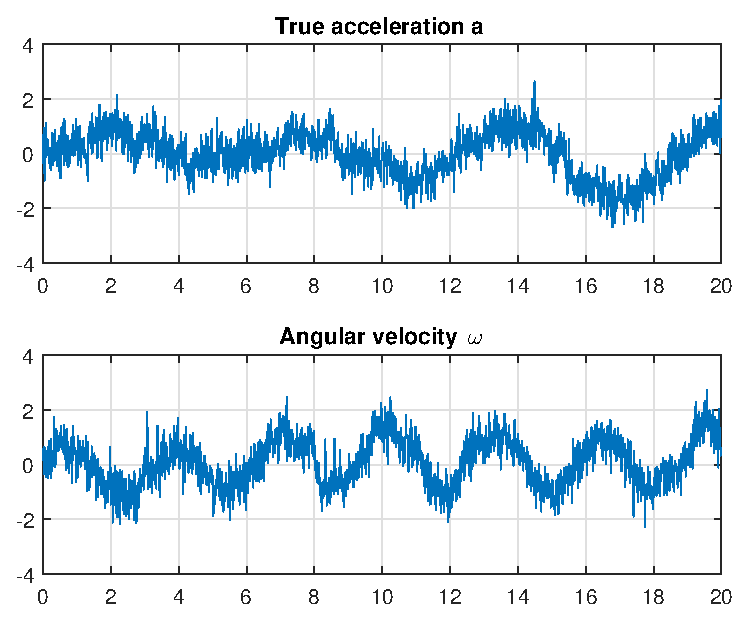
\includegraphics[width=1.25\textwidth, keepaspectratio=true]{../src/task1.eps}}
    \caption{True acceleration and angular velocity.}
\end{figure}

\section*{Task 2}
In order to discretize the system, it must first be written as a state space model. The system

\begin{subequations}
\begin{equation}
	\dot{x} = v 
\end{equation}
\begin{equation}
	\dot{v} = a
\end{equation}
\begin{equation}
	\dot{\theta} = \omega
\end{equation}
\end{subequations}

can be written as

\begin{subequations}
\begin{equation}
	\dot{\bm{x}} = \bm{A}\bm{x} + \bm{B}\bm{u}
\end{equation}
\begin{equation}
	\begin{bmatrix}
		\dot{x} \\ \dot{v} \\ \dot{\theta}
	\end{bmatrix}
	=
	\begin{bmatrix}
		0 & 1 & 0 \\
		0 & 0 & 0 \\
		0 & 0 & 0
	\end{bmatrix}
	\begin{bmatrix}
		x \\ v \\ \theta
	\end{bmatrix}
	+
	\begin{bmatrix}
		0 & 0 \\
		1 & 0 \\
		0 & 1
	\end{bmatrix}
	\begin{bmatrix}
		a \\ \omega
	\end{bmatrix}
	.
\end{equation}
\end{subequations}

By using forward Euler to discretize the system, it can be written on the form

\begin{equation}
	\label{eq:euler}
	\bm{x}(t_{k+1}) = (\bm{I} + h\bm{A}(t_k))\bm{x}(t_k) + h\bm{B}(t_k)\bm{u}(t_k)
\end{equation}

where $h$ is the step size. The discretized system then becomes

\begin{equation}
	\bm{x}(t_{k+1}) =
	\begin{bmatrix}
		1 & h & 0 \\
		0 & 1 & 0 \\
		0 & 0 & 1
	\end{bmatrix}
	\bm{x}(t_k) + 
	\begin{bmatrix}
		0 & 0 \\
		h & 0 \\
		0 & h
	\end{bmatrix}
	\bm{u}(t_k).
\end{equation}

Figure \ref{fig:disc_states} shows plots of the states in the discretized system.

\begin{figure}[!ht]
    \centering
    \makebox[\textwidth][c]{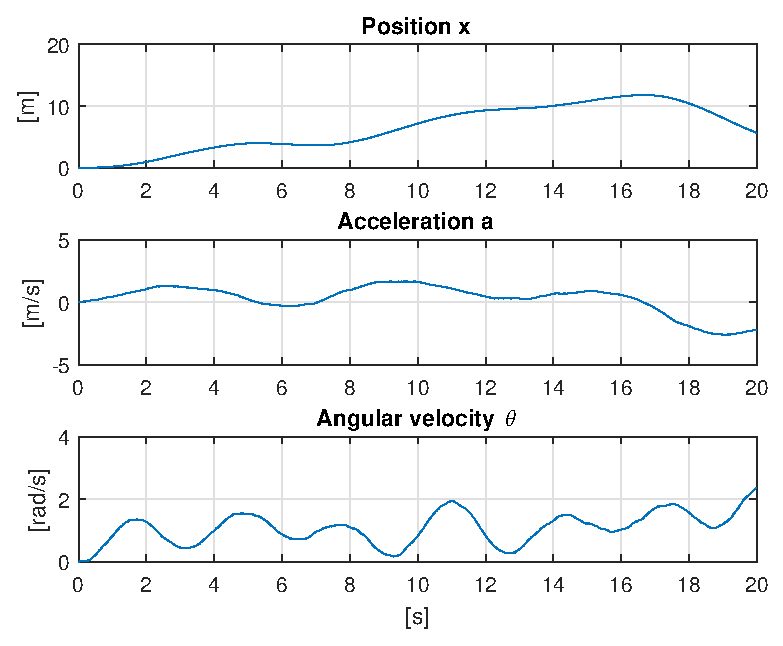
\includegraphics[width=1.25\textwidth, keepaspectratio=true]{../src/disc_states.eps}}
    \caption{States of the discretized system.}
    \label{fig:disc_states}
\end{figure}


\section*{Task 3}
When white noise is expressed in discrete time it is referred to as a white sequence \cite{heftet}, where the sequence consists of random variables that are uncorrelated \cite{wikiWhite}. The autocorrelation function for discrete white noise is:

\begin{equation}
	R_d(k) = A\delta(k) , \hspace{5pt} \delta(k) =
	\begin{cases}
		1 \hspace{10pt} k = 0 \\
		0 \hspace{10pt} k \neq 0
	\end{cases}.
\end{equation}

When using Matlab, white Gaussian noise can be generated by using \texttt{wgn()}, which will generate a sequence of uncorrelated random variables, which can be regarded as a white sequence.

The biases $b_1$ and $b_2$ can be discretized with forward Euler using equation \ref{eq:euler} from task 2. The bias can be written in state space form as

\begin{equation}
	\dot{\bm{x}} = 
	\begin{bmatrix}
		-\frac{1}{T_1} & 0 \\
		0 & -\frac{1}{T_2}
	\end{bmatrix}
	\bm{x} +
	\begin{bmatrix}
		1 & 0 \\
		0 & 1
	\end{bmatrix}
	\bm{w}
\end{equation}

where

\begin{center}
\begin{math}
	\bm{x} =
	\begin{bmatrix}
		b_1 \\ b_2
	\end{bmatrix}
	, \hspace{5pt} \bm{w} =
	\begin{bmatrix}
		w_1 \\ w_2
	\end{bmatrix}
	.
\end{math}
\end{center}

The resulting discretized system is:

\begin{equation}
	\bm{x}(t_{k+1}) =
	\begin{bmatrix}
		1 - \frac{h}{T_1} & 0 \\
		0 & 1 - \frac{h}{T_2}
	\end{bmatrix}
	\bm{x}(t_k) +
	\begin{bmatrix}
		h & 0 \\
		0 & h
	\end{bmatrix}
	\bm{w}(t_k).
\end{equation}

\begin{figure}[!ht]
    \centering
    \makebox[\textwidth][c]{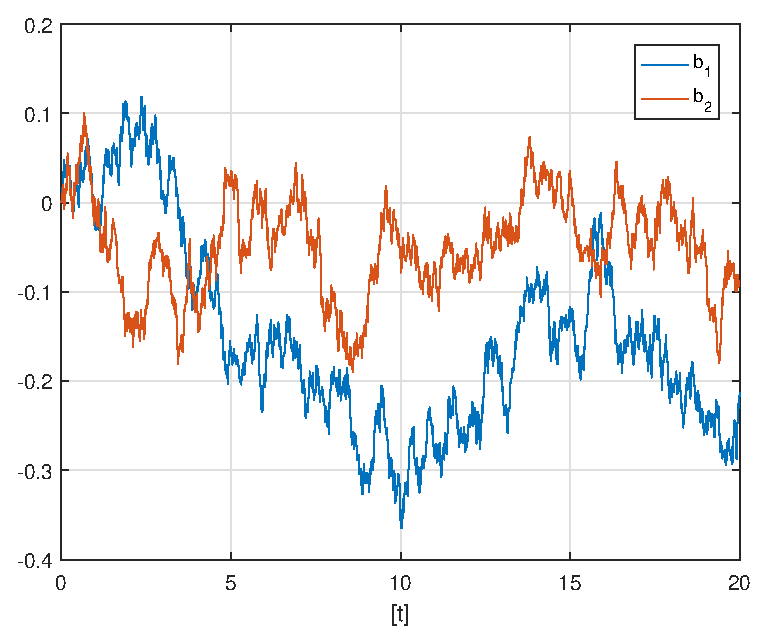
\includegraphics[width=1.25\textwidth, keepaspectratio=true]{../src/disc_bias.eps}}
    \caption{Bias modelled as a Gauss-Markov process.}
    \label{fig:disc_bias}
\end{figure}

\begin{figure}[!ht]
    \centering
    \makebox[\textwidth][c]{\includegraphics[width=1.25\textwidth, keepaspectratio=true]{../src/acc_pos_task3.eps}}
    \caption{Measured position and acceleration.}
\end{figure}

\begin{figure}[!ht]
    \centering
    \makebox[\textwidth][c]{\includegraphics[width=1.25\textwidth, keepaspectratio=true]{../src/angle_task3.eps}}
    \caption{Measured orientation angle and angular velocity.}
\end{figure}

\section*{Task 4}
The Kalman filter consists of several equations, which can be found in table 4.1 in \cite{heftet}.

The states for the Kalman filter are

\begin{equation}
	\bm{x} =
	\begin{bmatrix}
		x \\ v \\ b_1 \\ \theta \\ b_2
	\end{bmatrix}
	, \hspace{5pt} u = 
	\begin{bmatrix}
		a \\ \omega
	\end{bmatrix}
	, \hspace{5pt} y = 
	\begin{bmatrix}
		y_1 \\ y_2
	\end{bmatrix}
\end{equation}

The continous Kalman filter can be written as

\begin{equation}
	\dot{\hat{\bm{x}}} = \bm{A}\hat{\bm{x}} + \bm{B}\bm{u} + \bm{K}(\bm{y}-\bm{H}\hat{\bm{x}})
\end{equation}

where

\begin{center}
\begin{math}
	\hat{\bm{x}} = 
	\begin{bmatrix}
		\hat{x} \\ \hat{v} \\ \hat{b_1} \\ \hat{\theta} \\ \hat{b_2}
	\end{bmatrix}
	, \bm{A} = 
	\begin{bmatrix}
		0 & 1 & 0 & 0 & 0 \\
		0 & 0 & 1 & 0 & 0 \\
		0 & 0 & -\frac{1}{T_1} & 0 & 0 \\
		0 & 0 & 0 & 0 & 1 \\
		0 & 0 & 0 & 0 & -\frac{1}{T_2}
	\end{bmatrix}
\end{math}
\begin{math}
	\bm{B} = 
	\begin{bmatrix}
		0 & 0 \\
		1 & 0 \\
		0 & 0 \\
		0 & 1 \\
		0 & 0
	\end{bmatrix}
	, \bm{H} = 
	\begin{bmatrix}
		1 & 0 & 0 & 0 & 0 \\
		0 & 0 & 0 & 1 & 0
	\end{bmatrix}
\end{math}
\end{center}

When the system is discretized it will take the form

\begin{subequations}
\begin{equation}
	x(k+1) = \bm{\Phi}(k) \bm{x}(k) + \bm{\Updelta}(k) \bm{u}(k) + \bm{\Gamma}\bm{w}(k)
\end{equation}
\begin{equation}
	y(k) = \bm{H}(k)\bm{x}(k)+\bm{v}(k)
\end{equation}
\end{subequations}

Which gives

\begin{subequations}
\begin{equation}
	\bm{\Phi} = I + h\bm{A}(t_k)
\end{equation}
\begin{equation}
	\bm{\Updelta}(k) = h\bm{B}(t_k)
\end{equation}
\begin{equation}
	\bm{\Gamma}(k) = \bm{E}
\end{equation}
\end{subequations}

The design matrices of the Kalman filter, $\bm{Q}$ and $\bm{R}$, are chosen based on knowledge about the noise that is present in the system, namely the variance of the process noise and the measurement noise:

\begin{equation}
	\bm{Q}_d(k) = 
	\begin{bmatrix}
		Var(w_1) & 0 & 0 & 0 \\
		0 & Var(w_2) & 0 & 0 \\
		0 & 0 & Var(w_3) & 0 \\
		0 & 0 & 0 & Var(w_4)
	\end{bmatrix}
	, \hspace{5pt} \bm{R}_d(k) = 
	\begin{bmatrix}
		Var(v_1) & 0 \\
		0 & Var(v_2)
	\end{bmatrix}.
\end{equation}

And they are discretized

\begin{equation}
	\bm{Q}_d = h\bm{Q}
	, \hspace{5pt}
	\bm{R}_d = \frac{1}{h}
\end{equation}

The initial condistions of the filter are chosen as

\begin{subequations}
\begin{equation}
	\bar{\bm{x}}(0) = \bm{x}_0
\end{equation}
\begin{equation}
	\bar{\bm{P}}(0) = E[(\bm{x}(0)-\hat{\bm{x}}(0))(\bm{x}(0)-\hat{\bm{x}}(0))^T] = \bm{P}_0.
\end{equation}
\end{subequations}
	
The Kalman gain matrix is calculated by

\begin{equation}
	\bm{K}(k) = \bar{\bm{P}}(k)\bm{H}^T(k)[\bm{H}(k)\bar{\bm{P}}(k)\bm{H}^T(k) + \bm{R}_d(k)]^{-1}
\end{equation}

and the state estimation performed at every timestep is defined as

\begin{equation}
	\hat{\bm{x}}(k) = \bar{\bm{x}}(k) + \bm{K}(k)[\bm{y}(k)-\bm{H}(k)\bar{\bm{x}}(k)].
\end{equation}
	
The error covariance update is defined as

\begin{equation}
	\hat{\bm{P}}(k) = [\bm{I}-\bm{K}(k)\bm{H}(k)]\bar{\bm{P}}(k)[\bm{I}-\bm{K}(k)\bm{H}(k)]^T+\bm{K}(k)\bm{R}_d(k)\bm{K}^T(k).
\end{equation}
	
The propagation of the system is updated in both the state estimation and the error covariance

\begin{subequations}
\begin{equation}
	\bar{\bm{x}}(k+1) = \bm{\Phi}(k)+\hat{\bm{x}}(k)+\Updelta(k)\bm{u}(k)
\end{equation}
\begin{equation}
	\bar{\bm{P}}(k+1) = \bm{\Phi}(k)\hat{\bm{P}}(k)\bm{\Phi}^T(k)+\bm{\Gamma}(k)\bm{Q}_d(k)\bm{\Gamma}^T(k).
\end{equation}
\end{subequations}

\begin{figure}[!ht]
    \centering
    \makebox[\textwidth][c]{\includegraphics[width=1.25\textwidth, keepaspectratio=true]{../src/kalman_task4.eps}}
    \caption{The estimated states.}
\end{figure}

\begin{figure}[!ht]
    \centering
    \makebox[\textwidth][c]{\includegraphics[width=1.25\textwidth, keepaspectratio=true]{../src/kalman_bias_task4.eps}}
    \caption{Estimated bias.}
\end{figure}


\section*{Task 5}
The difference between a direct and an indirect Kalman filter is that an indirect filter estimates the error of the measurements based on an error model. The error model for the three states $x$, $v$ and $\theta$ will in this case be \cite{heftet}:

\begin{subequations}
\begin{equation}
	\delta\dot{x} = \delta v
\end{equation}
\begin{equation}
	\delta\dot{v} = b_1 + w_1
\end{equation}
\begin{equation}
	\dot{b_1} = -\frac{1}{T_1}b_1 + w_2
\end{equation}
\begin{equation}
	\delta\dot{\theta} = b_2 + w_3
\end{equation}
\begin{equation}
	\dot{b_2} = -\frac{1}{T_2}b_2 + w_4
\end{equation}
\end{subequations}

These error models will together form the following states for the Kalman filter

\begin{equation}
	\hat{\bm{x}} =
	\begin{bmatrix}
		\delta\hat{x} \\ \delta\hat{v} \\ \hat{b_1} \\ \delta\hat{\theta} \\ \hat{b_2}
	\end{bmatrix}
	, \hspace{5pt}
	\bm{y} = 
	\begin{bmatrix}
		x_{GPS} - x_{INS} + v_1 \\
		\theta_{GPS} - \theta_{INS} + v_2
	\end{bmatrix}
\end{equation}

which together will form the Kalman equation

\begin{equation}
	\dot{\hat{\bm{x}}} = \bm{\Phi}\hat{\bm{x}} + \bm{K}(\bm{y} - \bm{H}\hat{\bm{x}})
\end{equation}

The $\Phi$, $\bm{\Updelta}$, $\bm{H}$ and $\bm{\Gamma}$ matrices will stay the same as in the previous task, as will the design matrices $\bm{Q}$ and $\bm{R}$.
	
\begin{figure}[!ht]
    \centering
    \makebox[\textwidth][c]{\includegraphics[width=1.25\textwidth, keepaspectratio=true]{../src/kalman_task5.eps}}
    \caption{The estimated states}
\end{figure}

\begin{figure}[!ht]
    \centering
    \makebox[\textwidth][c]{\includegraphics[width=1.25\textwidth, keepaspectratio=true]{../src/kalman_bias_task5.eps}}
    \caption{Estimated bias.}
\end{figure}
	

\newpage
\addcontentsline{toc}{chapter}{References}
\begin{thebibliography}{25}

	\bibitem{heftet}
	Vik, Bjørnar (2014)
	\emph{"Integrated Satellite and Inertial Navigation Systems"},
	Norwegian University of Science and Technology, Department of Engineering Cybernetics, Trondheim
	
	\bibitem{wikiWhite}
	Wikipedia,
	\emph{https://en.wikipedia.org/wiki/White\_noise},
	accessed 05.11.2016
	
\end{thebibliography}

\end{document}